\documentclass{article}
\usepackage{polski}
\usepackage[utf8]{inputenc}
\usepackage{graphicx}
\usepackage[a4paper, total={7in, 10in}]{geometry}
\usepackage{listings}
\usepackage{amsmath}
\usepackage{stackengine}
\usepackage{subcaption}
\usepackage{float}
\usepackage{graphicx}
\renewcommand{\vec}[1]{\mathbf{#1}}
\usepackage[section]{placeins}
\graphicspath{ {./images/} }

\title{Zastosowanie Qlearningu w zachowaniu boidów}
\author{Jakub Łęcki, Marek Hering, Maciej Jabłoński}
\date{08.06.2020}
\begin{document}
\maketitle
\begin{abstract}
    Tematem niniejszej pracy jest problem nauczenia boidów (w naszym przypadku są to ryby), aby poprzez prawidłowe poruszanie się maksymalizowały swój czas życia. W tym celu użyliśmy koncepcji qlearningu oraz algorytmu stada.
\end{abstract}

\section{Boidy}
\subsection{Pochodzenie}
Termin \textbf{boid} został stworzony przez Craiga Reynoldsa w 1987 roku jako określenie stworzenia wykazującego cechy stadne. Słowo boid wzięło się z uproszeczenia terminu 'bird-like' jako odniesienie do ptaków formujących się w gromady.
\subsection{Zasady zachowania}
\label{sec:flocking_behavior}
Okazuje się, że w świecie rzeczywistym wiele gatunków zwierząt łączących się w grupy wykazuje podobne własności. Patrząc na stada ptaków, ławice ryb, roje pszczół lub stada owiec można zauważyć, że każda z jednostek stosuje się do 3 podstawowych zasad:
\begin{enumerate}
    \item Rozdzielność - osobnik nie lubi przebywać w tłoku, dlatego zachowuje dystans do swoich sąsiadów
    \item Spójność - osobnik nie lubi przebywać w samotności, więc kieruje się ku najbliższym współstadnikom 
    \item Wyrównanie - osobnik porusza się w kierunku zbliżonym do kierunku otaczających członków stada
\end{enumerate}

Łącząc te 3 proste zasady, boidy tworzą złożone i bardzo zorganizowane skupiska, które obserwujemy jako np. ławice ryb, które pozostają w płynnym, nieustannym ruchu.
\section{Qlearning}
Jest to jedna z technik szerokiej dziedziny uczenia maszynowego znanej jako "Uczenie ze wzmocnieniem" (ang. Reinforcement Learning). Opiera się na śledzeniu zachowania agentów oraz efektów, które owe akcje powodują. W tym celu używana jest tablica stanów-akcji zwykle nazywana jako \textbf{qtable}.
\subsection{Qtable}
Tablica ma wymiary m \(\times\) n, gdzie:
\begin{itemize}
    \item m - liczba możliwych stanów
    \item n - liczba akcji możliwych do wykonania 
\end{itemize}

W każdej komórce \(Q(s,a)\) znajduje się oczekiwana wartość nagrody jaką agent otrzyma będąc w stanie \(s\) i wykonawszy akcję \(a\). Po wykonaniu akcji, agent przechodzi do kolejnego stanu \(s'\).
Agent będąc w stanie \(s\) będzie wybierać swoją kolejną akcję na podstawie polityki \(argmax(Q(s))\), czyli wybranie akcji za którą teoretycznie otrzyma największą nagrodę.
\subsection{Środowisko}
Jest to zbiór agentów oraz dowolnych innych encji z którymi agent może w jakiś sposób oddziałowywać. Rolą środowiska jest wykonanie akcji wybranej przez agenta i ocenienie jak dobrze akcja została wybrana. W tym celu środowisko nadaje agentowi nagrody (i kary, jeśli nagroda jest ujemna). W kolejnych rundach skutkuje to stopniowym poprawianiem procesu wyboru akcji i agent zbiera coraz wyższe nagrody. Po wykonaniu kroku środowisko przekazuje do algorytmu uczenia zestaw danych:
\begin{itemize}
    \item stan w którym był agent
    \item akcja jaką wykonał
    \item stan w którym znajduje się po wykonaniu akcji
    \item nagroda jaką otrzymał za przejście do kolejnego stanu
\end{itemize}
\subsection{Proces uczenia}
Aby agent wybierał z czasem coraz lepsze decyzje, wartości w Qtable muszą ulegać zmianie. Odbywa się to w oparciu o poniższe równanie:
\begin{equation}
    \label{eqn:bellman_equation}
    Q'(s, a)\leftarrow Q(s, a) + \alpha \cdot\left(r  + \gamma\cdot \stackunder{max}{a} Q(s', a) - Q(s,a) \right) 
\end{equation}
Gdzie \(s\) i \(a\) to stan i akcja przed jej wykonaniem, a  \(s'\) to stan po wykonaniu akcji.
\subsubsection{Współczynnik uczenia \(\alpha\)}
Wartość \(\alpha \in <0, 1>\) reguluje jak bardzo znacząca jest nowa informacja uzyskana w wyniku wykonania akcji w środowisku. Przy wartości 0 agent nie będzie się uczył niczego nowego, natomiast przy \(\alpha = 1\) agent zaakceptuje całą zdobytą wiedzę. 
\subsubsection{Współczynnik dyskontowania \(\gamma\)}
Wartość \(\gamma \in <0, 1>\) określa ważność przyszłych nagród zdobywanych przez agenta. Wartość dążąca do zera zwiększy sugerowanie się pamięcią krótkotrwałą, natomiast do 1 pamięcią długotrwałą. Ważnym elementem jest, aby \(\gamma\) rzeczywiście zawierała się w przedziale \(<0, 1)\) ponieważ zapewnia to zbieżność wartości przewidywanej nagrody. Jeśli proces uczenia byłby nieskończony i \(\gamma \ge 1\) (a nawet lekko poniżej) wartości nagród rosłyby nieustannie zaburzając proces.
\subsubsection{Efekt}
W wyniku przeprowadzenia odpowiedniej ilości kroków wartości nagród zbiegają się do optymalnych, a w tabeli powstają zależności pomiędzy poszczególnymi stanami umożliwiające dotrzeć do nawiększej nagrody, dysponując jedynie obecnym stanem i przewidywaną nagrodą.
\subsubsection{Polityka wspomagająca}
Gdy podczas uczenia agent będzie słuchał się tylko tabeli qlearningu, może się zdarzyć że zadowoli się częściowo poprawnym rozwiązaniem, zamiast szukać rozwiązania dokładnego. Aby uniknąc takiej sytuacji proces wybierania akcji rozszerza się często o politykę \textbf{epsilon greedy}, w której z pewnym prawdopodobieństwem wybierana jest losowa akcja zamiast wskazywanej przez tabelę. Wartość \(\epsilon\) jest zmniejszana z czasem, aby agent coraz częściej stosował to czego się nauczył.

\section{Kontrola ruchu boidów}
\subsection{Ruch ciągły}
Boidy muszą być osadzone w przestrzeni euklidesowej, zatem każdy z boidów posiada trzy dwuwymiarowe wektory położenia, prędkości i przyspieszenia.\\
Aby agent mógł poruszać się ruchem gładkim, postanowiliśmy kontrolować boidy za pomocą przyspieszenia, a na prędkość nałożyć ograniczenia w postaci minimalnej i maksymalnej wartości.
\subsection{Stan agenta}
Stanem agenta jest jego pozycja oraz kąt nachylenia prędkości do osi X. 
\subsection{Dyskretyzacja}
Qlearning z definicji działa na wartościach dyskretnych, ponieważ wartości nagród wpisujemy pod konkretne wiersze i kolumny tabeli. Zatem konieczne było zdyskretyzowanie stanu agenta. Wykonaliśmy to poprzez przeniesienie pozycji agenta w przestrzeń o dużo mniejszej rozdzielczości \(r\), a kąt spłaszczamy do \(N\) równo oddalonych wartości.
\subsection{Akcja agenta}
W klasycznym algorytmie qlearningu na wyjściu otrzymujemy \(N\) wartości nagród, spośród których indeks maksymalnej wartości symbolizuje akcję do wykonania. W naszym problemie jednak sprowadzenie ruchu do zaledwie kilku kierunków nie spełniłoby założenia o gładkości, dlatego przyjęliśmy nową politykę. Zamiast wyznaczać przyśpieszenie na podstawie jednej akcji, wyznaczamy je według wzoru:
\begin{equation}
    a = \sum \limits_{i = 0}^{N}a_i
\end{equation}
gdzie \(i\) to indeks akcji, \(N\) to ilość możliwych kierunków, natomiast \(a_i\) to wektor w postaci biegunowej: 
\begin{equation}
    a_i = [r_i, i \cdot 360/N]
\end{equation}
gdzie \(r_i\) to wartość nagrody otrzymanej za i-tą akcję.\\
Użycie wartości nagrody poskutkuje poprawną reakcją boida ponieważ w miejscach których ma unikać nagroda będzie ujemna, a w możliwych do przemieszczenia - dodatnia.
\section{Utrzymanie agentów na planszy}

\begin{figure}[H]
    \centering
    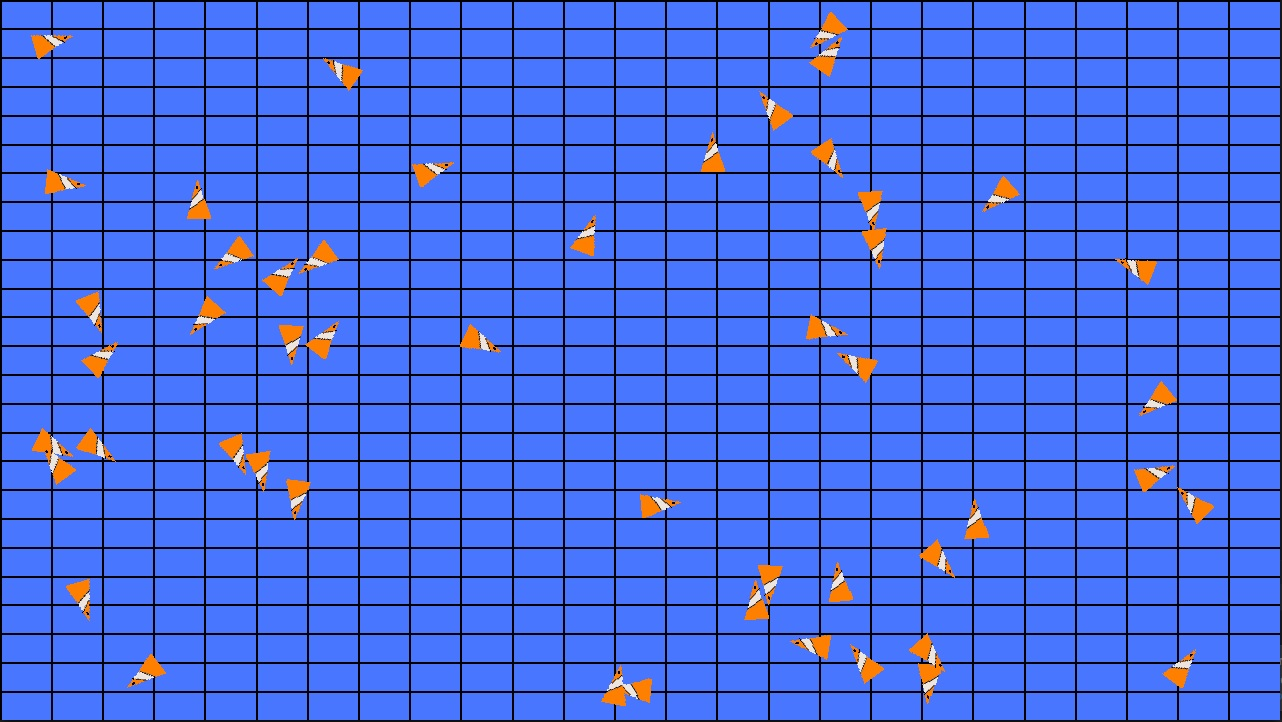
\includegraphics[width=0.75\textwidth]{1_Qtable_init.jpg}
    \caption[]{Stan początkowy planszy z agentami. Siatka symbolizuje komórki qtable zależne od położenia}
\end{figure}
Na początku zajęliśmy się nauczeniem boidów, aby nie dotykały krawędzi. W tym celu przyjęliśmy rozdzielczość tablicy stanów \(25\times25\) oraz 12 kierunków w których możliwe jest obliczenie przyśpieszenia.\\
Dodatkowo:
\begin{enumerate}
    \item ilość ryb = 50
    \item długość epoki = 2000 klatek (\(\approx\) 1 min)
\end{enumerate}
\subsection{Nagradzanie}
Boid za dotknięcie granicy otrzymuje nagrodę o wysokości -1000.
\subsection{Wynik}
Boidy dość skutecznie utrzymywały się przy życiu, jednak ich ruch bardziej przypominał odbijanie się niż omijanie krawędzi. Wynika to z faktu, że nagroda wyznaczana jest tylko w tej komórce w której agent zginie, nie ma żadnej relacji pomiędzy sąsiednimi stanami, więc reakcja następowała tylko tuż przy granicy.
\subsection{Modyfikacja polityki aktualizacji tablicy stanów}
\label{sec:politics_modification}
W tradycyjnym algorytmie qlearningu, równanie (\ref{eqn:bellman_equation}) Bellmana aktualizuje stan przez wybranie maksymalnej nagrody możliwej do uzyskania. W naszym przypadku nie jest to skuteczne, ponieważ wykonanie akcji nie skutkuje natychmiastowym uzyskaniem nagrody. Aby umożliwić agentowi ocenienie czy warto ruszyć się w danym kierunku zrezygnowaliśmy z wybierania wartości maksymalnej. Zamiast tego bierzemy wszystkie możliwe nagrody do uzyskania po wyjściu z obecnego stanu i liczymy średnią arytmetyczną z minimalnej i maksymalnej nagrody. Dzięki temu w tabeli stanów powstaje swego rodzaju dyskretne pole siłowe, które nadaje boidom kierunek w którym powinny się udać.
\subsection{Stan tabeli z nową polityką nagród} 
Po powyższej zmianie wyniki mają się następująco. Strzałki oznaczają kierunek wypadkowego przyśpieszenia.

\begin{figure}[H]
    \begin{minipage}[h]{0.48\textwidth}
        \centering
        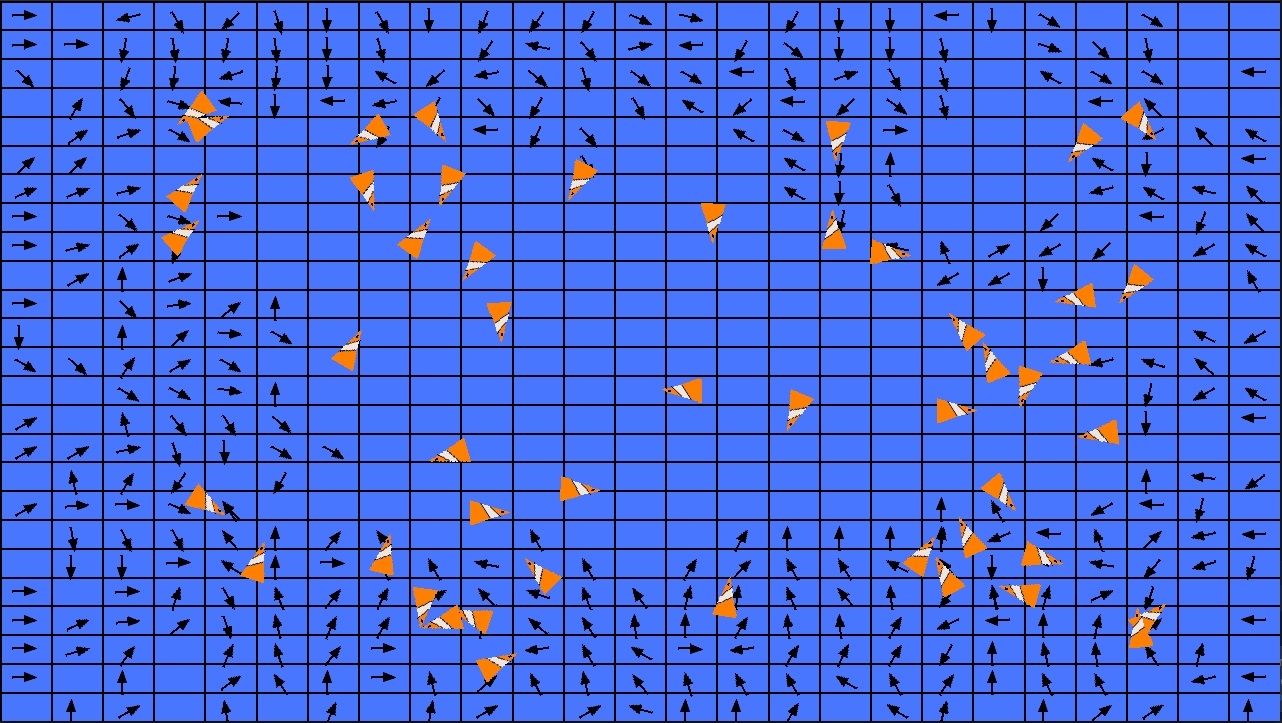
\includegraphics[width=\textwidth]{2_Qtable_after_2nd_epoch.jpg}
        \caption{Stan tabeli po dwóch epokach}
    \end{minipage}
    \hspace{0.02\textwidth}
    \begin{minipage}[h]{0.48\textwidth}
        \centering
        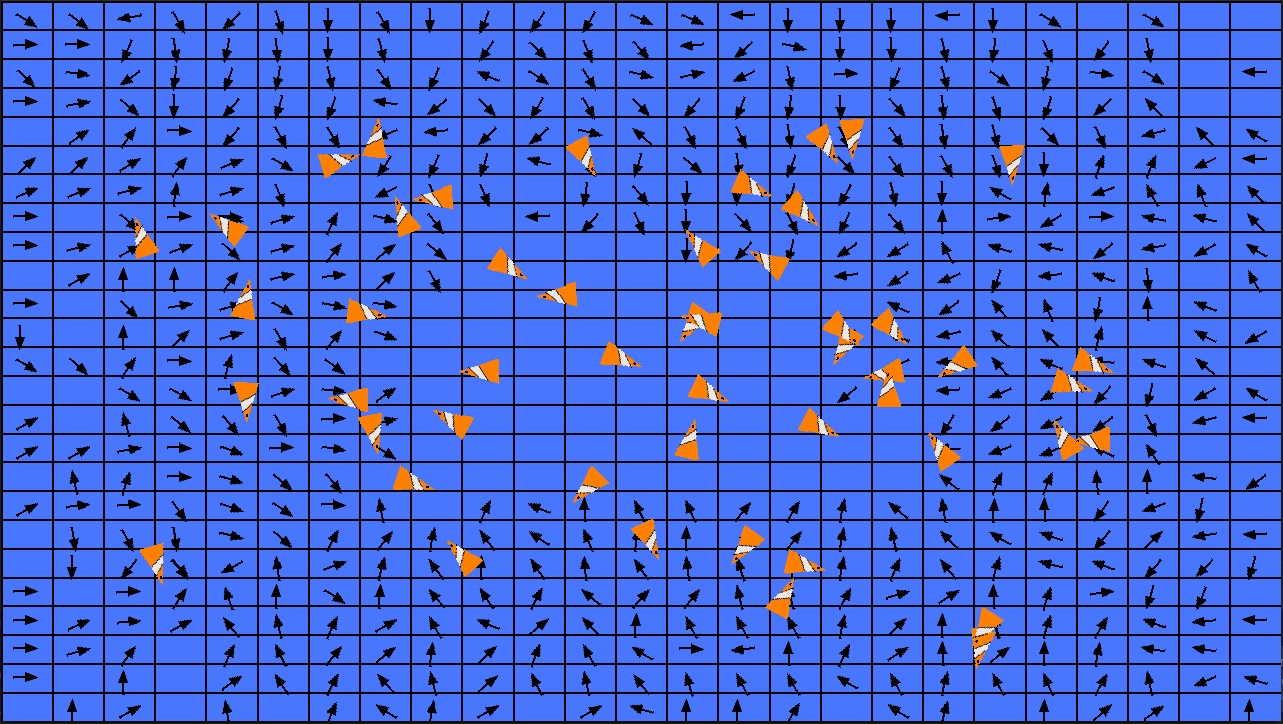
\includegraphics[width=\textwidth]{3_Qtable_after_3rd_epoch.jpg}    
        \caption{Stan tabeli po 3 epokach}
    \end{minipage}
\end{figure}
\begin{figure}[H]
    \begin{minipage}[h]{0.48\textwidth}
        \centering
        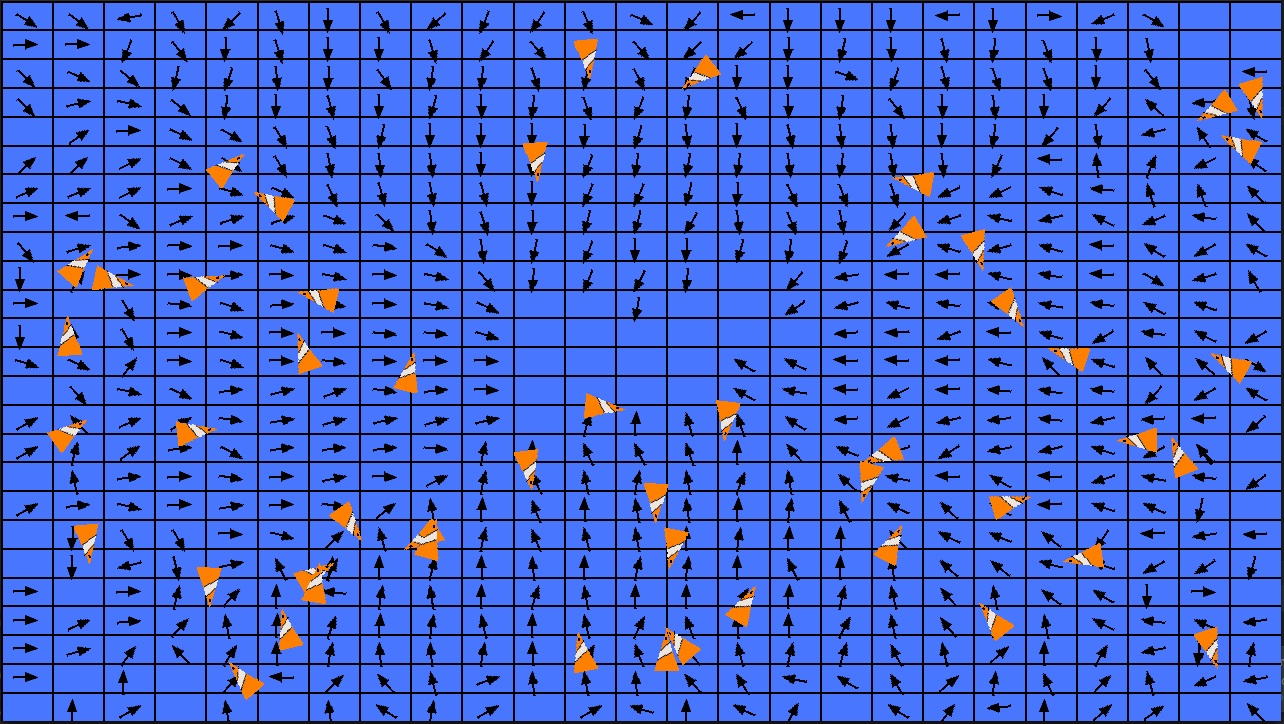
\includegraphics[width=\textwidth]{4_Qtable_after_5rd_epoch.jpg}
        \caption{Stan tabeli po 5 epokach}
    \end{minipage}
    \hspace{0.02\textwidth}
    \begin{minipage}[h]{0.48\textwidth}
        \centering
        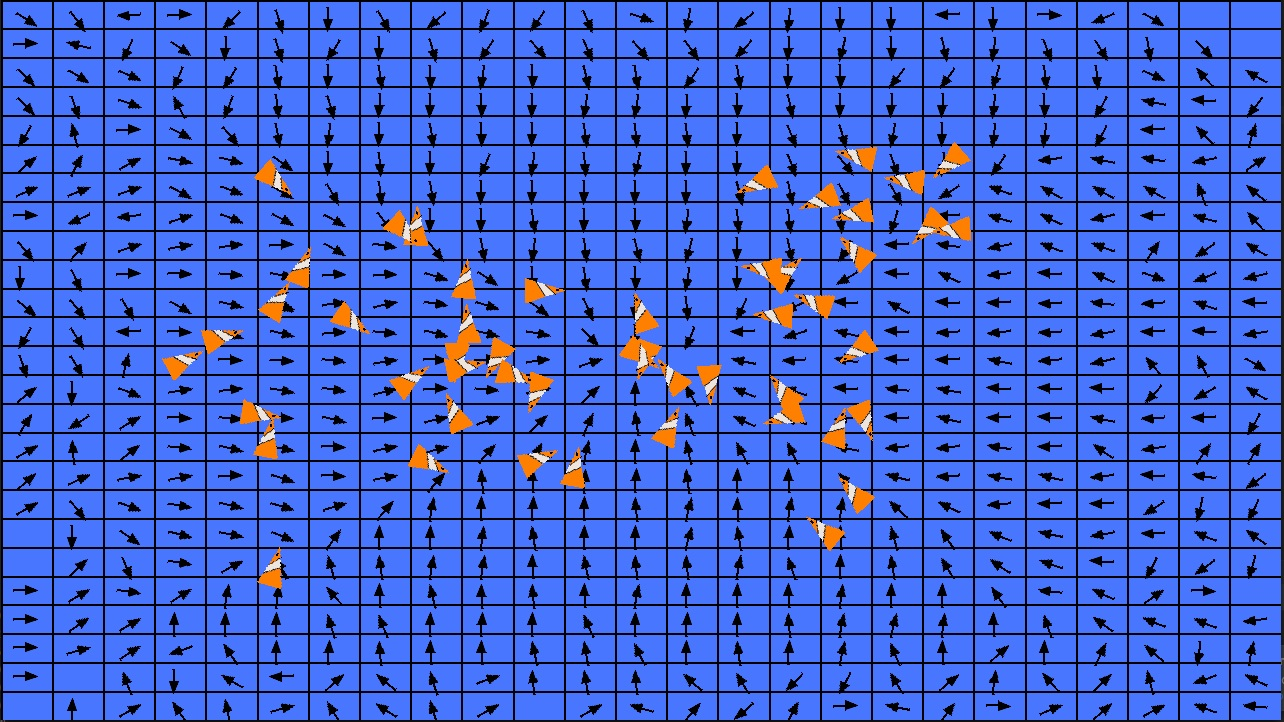
\includegraphics[width=\textwidth]{5_Qtable_after_10th_epoch.jpg}
        \caption{Stan tabeli po 10 epokach}
    \end{minipage}
\end{figure}

Jak widać już po 10 epokach agenci nauczyli się skutecznie unikać krawędzi. Patrząc na kierunki poszczególnych strzałek widzimy, że w tabeli powstało pole, które zbiega się do środka tworząc optymalne ścieżki nawet w nietrywialnych miejscach takich jak rogi planszy. Jest to bardzo korzystne, ponieważ takie miejsca sprawiają zawsze problem w algorytmicznym wykrywaniu kolizji.

\begin{figure}[H]
    \begin{minipage}{0.48\textwidth}
        \centering
        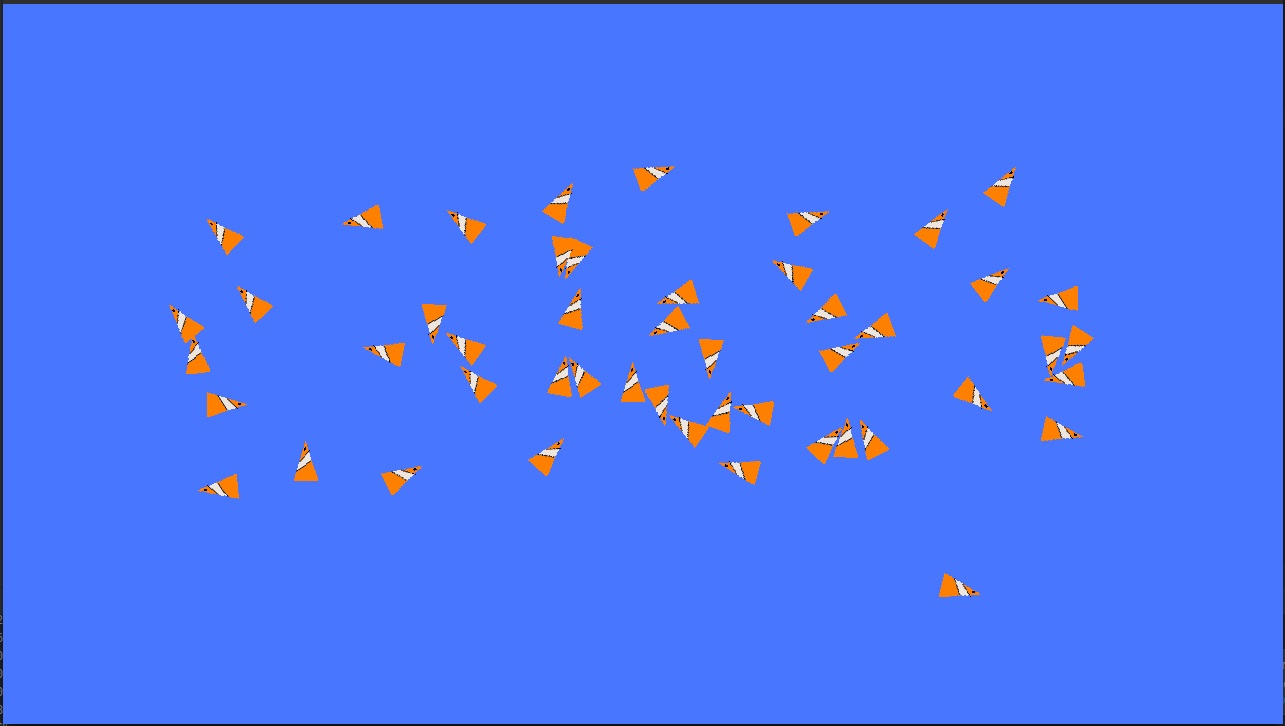
\includegraphics[width=\textwidth]{6_Learing_result.jpg}
        \caption{Ryby utrzymujące się na środku planszy po nauczeniu}
    \end{minipage}
    \hspace{0.02\textwidth}
    \begin{minipage}{0.48\textwidth}
        \centering
        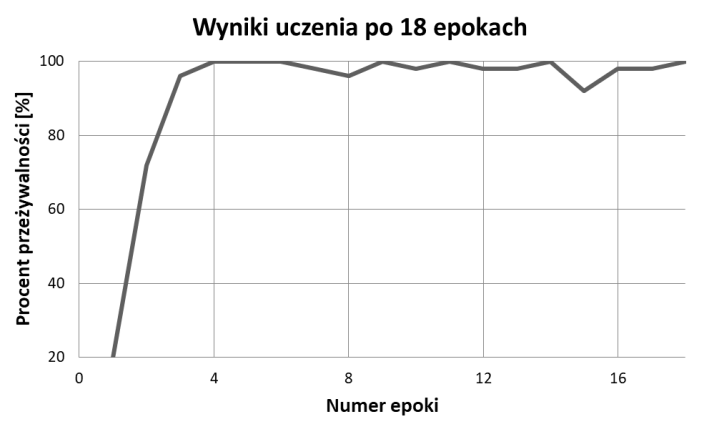
\includegraphics[width=\textwidth]{borders_learning_plot.png}
        \caption{Wykres przeżywalności ryb w czasie uczenia}
    \end{minipage}
\end{figure}
\section{Polowanie i uciekanie}
W kolejnym etapie postanowiliśmy dodać do środowiska boidy drugiego rodzaju, tzn. drapieżniki. Ich zadaniem jest manipulowanie swoim ruchem, aby zjadać ryby. W momencie kolizji drapieżnika z rybą następuje śmierć ryby. Drapieżniki tak samo jak ryby umierają na krawędziach planszy.
\subsection{Qtable}
Aby umożliwić nauczenie się zarówno uciekania jak i gonienia rozszerzyliśmy tablicę stanów o 2 wymiary. Jeden który indeksuje rodzaj uczącego się boida, drugi natomiast zawiera stany jako dyskretny kąt pod którym agent widzi swój cel. Celem odpowiednio jest najbliższa ryba dla drapieżnika i najbliższy drapieżnik dla ryby.
\subsection{Pole reakcji}
Odnajdywanie najbliższego celu dla każdego boida na planszy spośród wszystkich boidów ma istotne wady.
\begin{enumerate}
    \item Jest wysoce nieoptymalne, ponieważ wymaga przeszukania każdy z każdym więc ma czas \(O(n^2)\)
    \item Sugeruje, że boid posiada wiedzę \textit{a priori} o położeniu dowolnego innego boida, co nie pokrywa się z rzeczywistością,gdzie każdy organizm ma ograniczone pole widzenia i reakcji.
\end{enumerate}
W celu zasymulowania pola reakcji, każdy z boidów posiada poligon z regulowanym kątem widzenia, ograniczający odziaływanie pozostałych boidów tylko do tych które znajdują się wewnątrz wielokąta.
\begin{figure}[h]
    \centering
    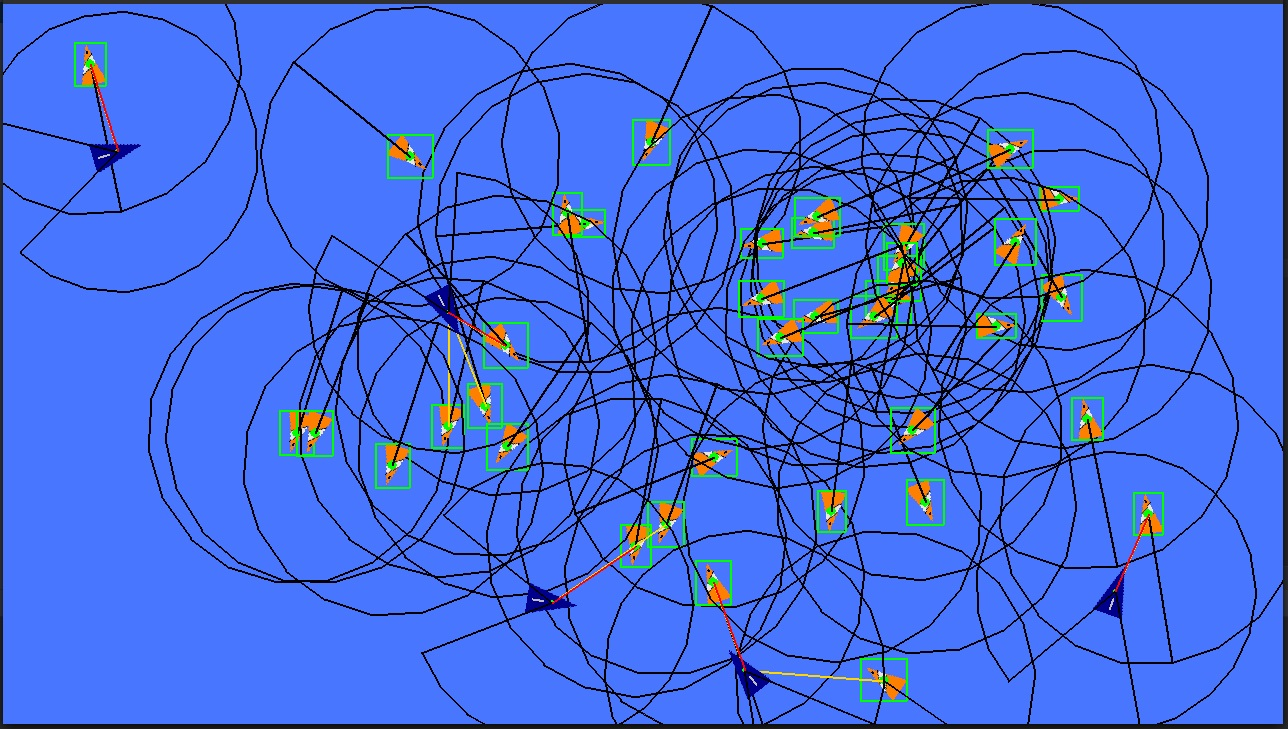
\includegraphics[width=0.7\textwidth]{12_hunting_debug.jpg}
    \caption{Przykładowy widok pól reakcji każdego z boidów}
\end{figure}
\begin{figure}[H]
    \begin{minipage}{0.48\textwidth}
        \centering
        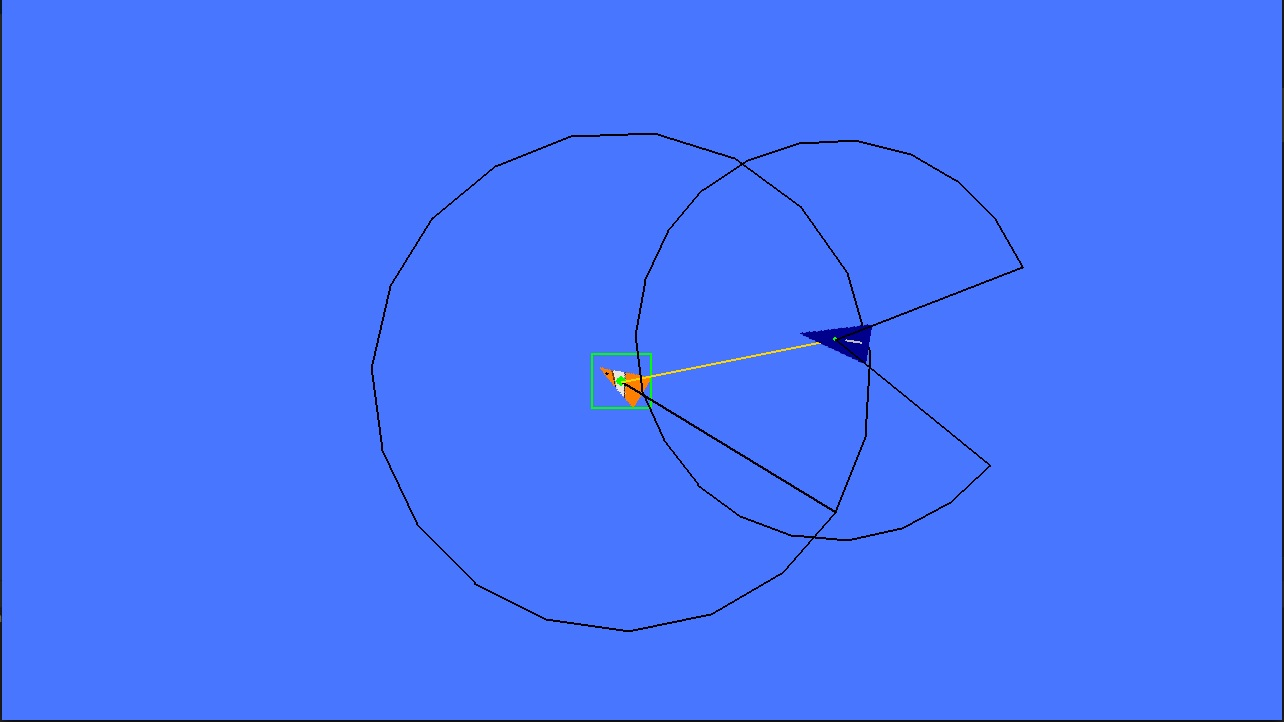
\includegraphics[width=\textwidth]{9_Fish_seeing_predator.jpg}
        \caption{Ryba, która widzi drapieżnika w swoim polu reakcji}
    \end{minipage}
    \hspace{0.02\textwidth}
    \begin{minipage}{0.48\textwidth}
        \centering
        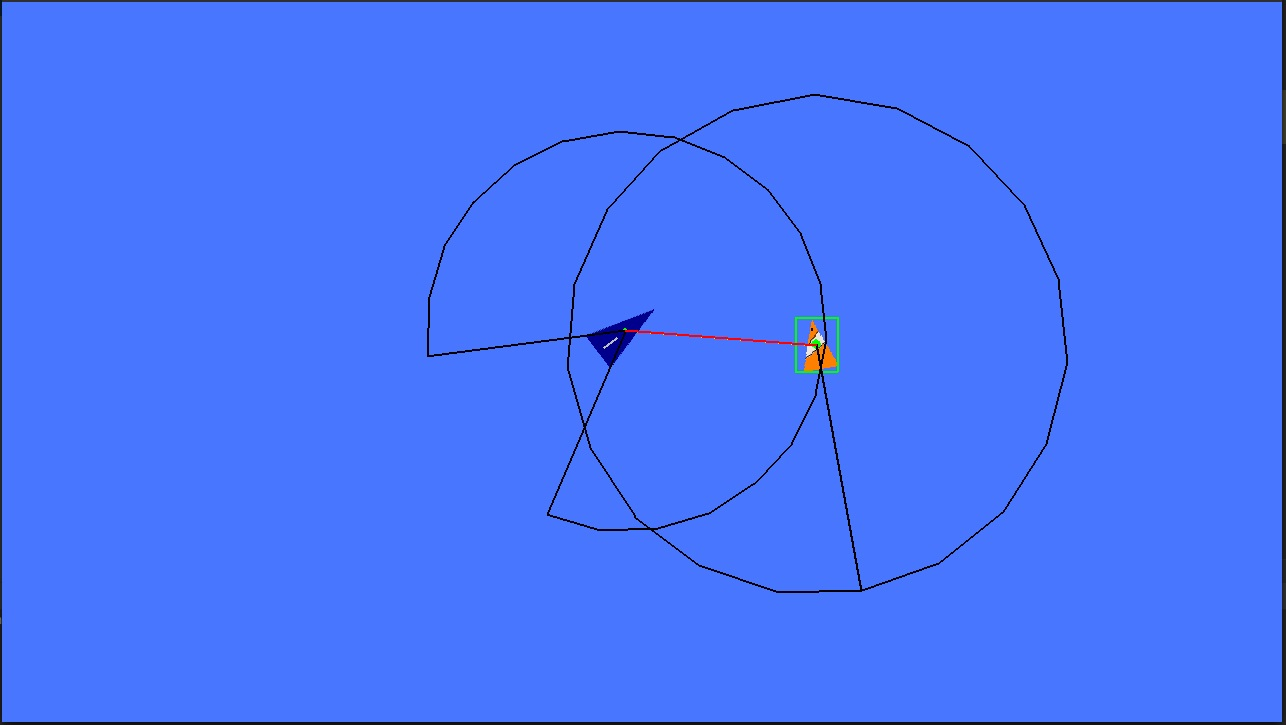
\includegraphics[width=\textwidth]{10_Predator_seeing_fish.jpg}
        \caption{Drapieżnik widzący rybę w soim polu reakcji}
    \end{minipage}
\end{figure}
\subsection{Proces uczenia}
Drapieżniki tak samo jak ryby muszą nauczyć się unikać krawędzi, zatem w pierwszej kolejności na planszy znajdowała się duża liczba drapieżników, aby szybko nauczyły się omijać granice planszy.
\begin{figure}[H]
    \begin{minipage}{0.48\textwidth}
        \centering
        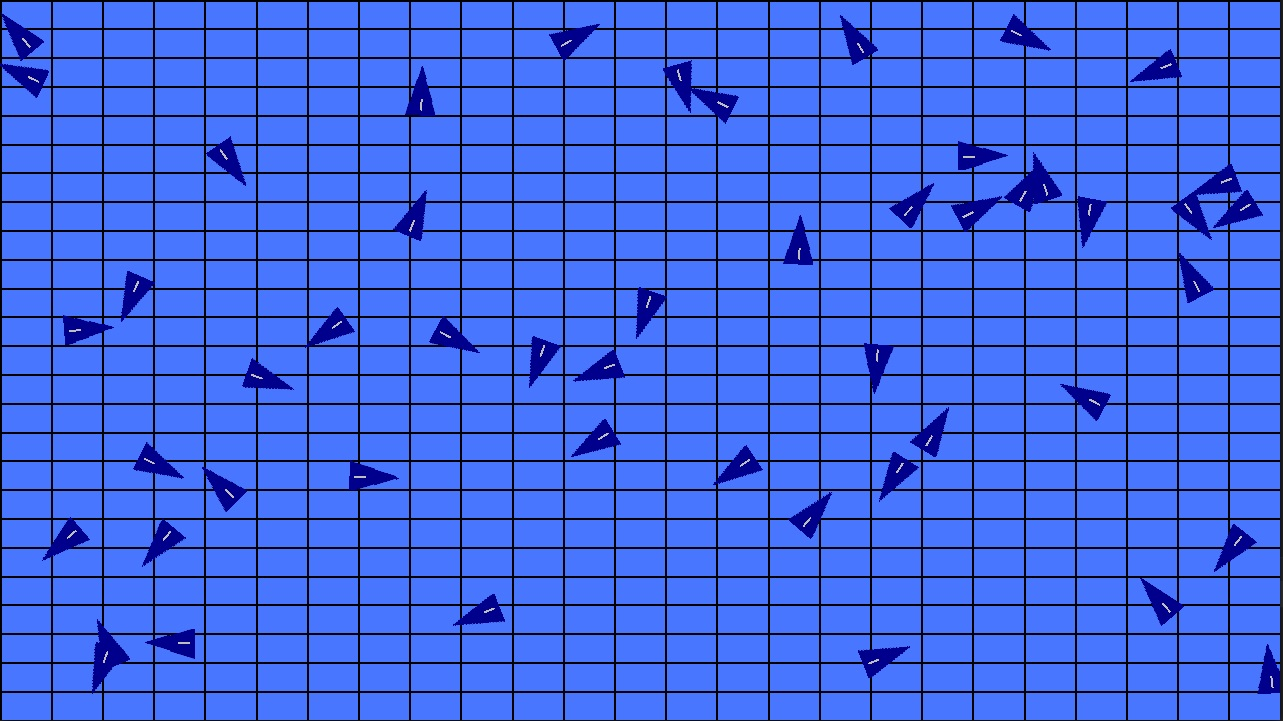
\includegraphics[width=\textwidth]{7_Predator_Qtable_init.jpg}
        \caption{Wizualizacja tablicy stanów drapieżników na początku uczenia}
    \end{minipage}
    \hspace{0.02\textwidth}
    \begin{minipage}{0.48\textwidth}
        \centering
        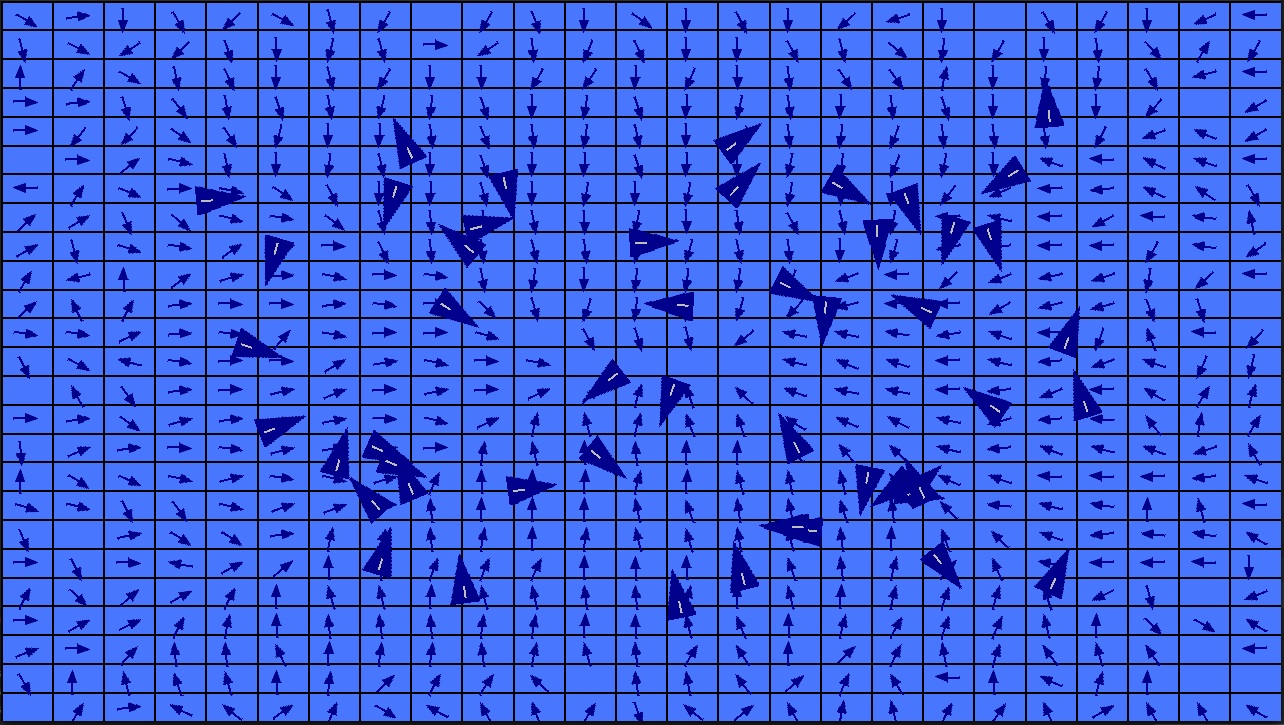
\includegraphics[width=\textwidth]{8_Predator_learning_result.jpg}
        \caption{Wizualizacja tablicy stanów po zakończonym uczeniu}
    \end{minipage}
\end{figure}
Jak widać na powyższym rysunku drapieżniki osiągają podobne wyniki do zwykłych ryb.
Kolejnym krokiem było dodanie ryb, które jednocześnie uczyły się omijać krawędzie, a także uciekać przed drapieżnikami. Drapieżniki natomiast umiejąc omijać już krawędzie mogły skupić się na doskonaleniu polowania.
\subsection{Nagrody}
Pozostawienie tylko jednej kary za śmierć o wartości -1000 było zbyt mało efektywne, dlatego dodaliśmy nagrodę dla drapieżnika za złapanie ryby w wysokości 500, oraz nagrody odpowiednio:
\begin{itemize}
    \item dla ryby nagroda z przedziału \(<-200, 200>\) proporcjonalna do kąta pomiędzy wektorem widzenia drapieżnika, a prędkością ryby
    \item dla drapieżnika kara z przedziału \(<-400, 400>\) proporcjonalna do kąta pomiędzy wektorem widzenia ryby, a prędkością drapieżnika
\end{itemize}
\subsection{Wyniki}
Po 50 epokach zarówno drapieżniki jak i ryby nauczyły się dosyć sprawnie poruszać i reagować na sytuację w otoczeniu. Przy 50 rybach i 4 drapieżnikach sytuacja wyglądała następująco.
\begin{figure}[H]
    \begin{minipage}{0.48\textwidth}
        \centering
        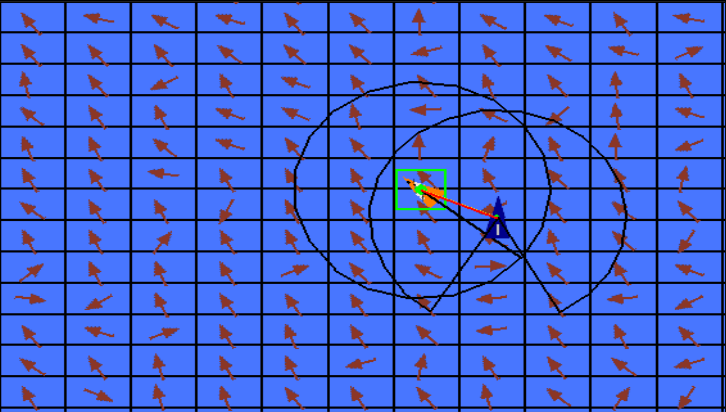
\includegraphics[width=\textwidth]{fish_being_followed.png}
        \caption{Ryba która widzi drapieżnika w prawym dolnym rogu}
    \end{minipage}
    \hspace{0.02\textwidth}
    \begin{minipage}{0.48\textwidth}
        \centering
        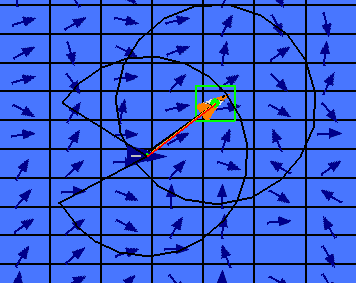
\includegraphics[width=\textwidth]{hunting_predator.png}
        \caption{Drapieżnik, który widzi rybę w prawym górnym rogu}
    \end{minipage}
    \caption{Wizualizacja tablicy stanów w zależności od kąta widzenia celu}
    \label{fig:angle_to_objective}
\end{figure}
Na ilustracji \ref{fig:angle_to_objective} widać w jaki sposób boid poruszałby się gdyby stosowałby się tylko do reakcji na cel. Oczywiście jednocześnie działa też unikanie krawędzi stąd boid zadziała pod wpływem wypadkowej siły.
\begin{figure}[H]
    \centering
    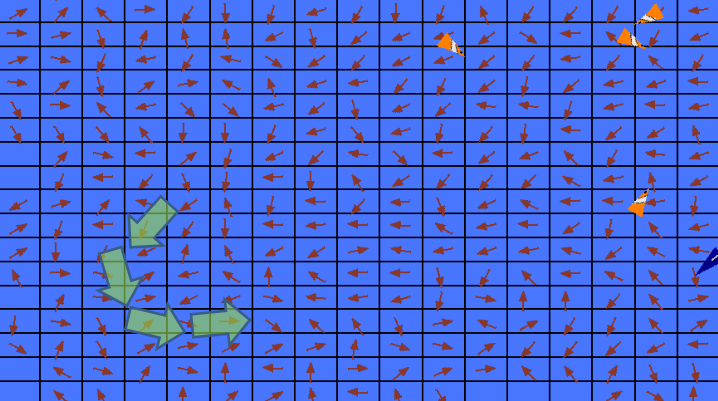
\includegraphics[width=0.7\textwidth]{possible_track.png}
    \caption{Możliwa droga, którą ryba będzie się przemieszczać kiedy będzie goniona od strony prawego górnego rogu}
\end{figure}
\begin{figure}[H]
    \begin{minipage}{0.48\textwidth}
        \centering
        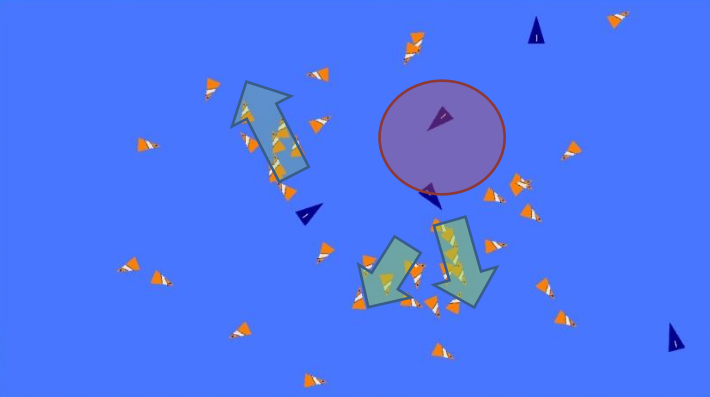
\includegraphics[width=\textwidth]{boid_opposite_direction.png}
        \caption{Ryby, które wykryją w swoim polu reakcji drapieżnika dobierają optymalny kierunek ucieczki.}
    \end{minipage}
    \hspace{0.02\textwidth}
    \begin{minipage}{0.48\textwidth}
        \centering
        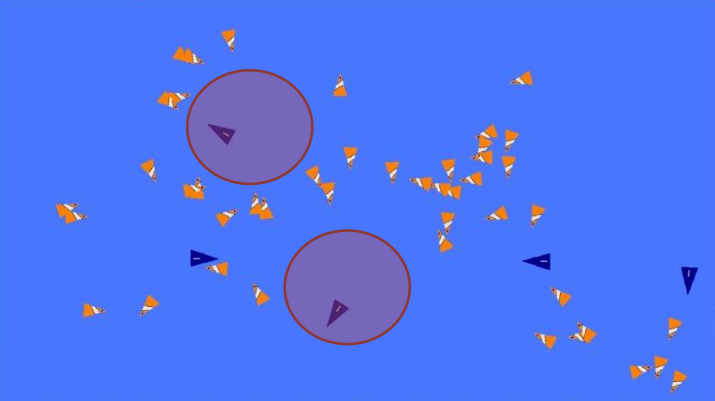
\includegraphics[width=\textwidth]{fish_fleeing.png}
        \caption{Drapieżnik odstrasza ryby, tworząc wokól siebie pustą przestrzeń.}
    \end{minipage}
\end{figure}
\section{Zachowanie ławicowe}
Ostatnim etapem naszego projektu było zaimplementowanie algorytmicznego zachowania ławicy wspomnianego w sekcji \ref{sec:flocking_behavior} oraz porównanie czy w połączeniu z qlearningiem wpływa korzystnie na zachowanie ryb.
\subsection{Implementacja}
Do wykrywania sąsiedztwa boida wykorzystaliśmy wcześniej przygotowane pole reakcji.
\subsubsection{Rozdzielność}
Zasada rozdzielności obliczana jest jako ujemna suma różnic pomiędzy położeniem najbliższym sąsiadów a boidem.
\begin{equation}
    \vec{s} = - \sum\limits_{i=1}^n( \vec{m_i} - \vec{p})
\end{equation}
gdzie \(m_i\) to pozycja i-tego sąsiada, \(p\) to pozycja obecnego boida, a \(n\) to ilość sąsiadów w polu reakcji.
\subsubsection{Spójność}
Zasada spójności liczona jest jako różnica pomiędzy średnim położeniem sąsiadów, a położeniem boida.
\begin{equation}
    \vec{c} = \frac{1}{n} \cdot \sum\limits_{i=1}^n \vec{m_i} - \vec{p}
\end{equation}
gdzie \(m_i\) to pozycja i-tego sąsiada, \(p\) to pozycja obecnego boida, a \(n\) to ilość sąsiadów w polu reakcji.
\subsubsection{Wyrównanie}
Zasada wyrównania obliczana jest jako różnica pomiędzy średnią prędkością sąsiadów,  a prędkością boida.
\begin{equation}
    \vec{a} = \frac{1}{n}\cdot\sum\limits_{i=1}^{n}\vec{v_i} - \vec{v}
\end{equation}
gdzie \(v\) to prędkość boida, \(v_i\) prędkość i-tego sąsiada, a \(n\) to ilość sąsiadów w polu reakcji.
\subsubsection{Wypadkowa}
Końcowy wektor sterujący boidem w ławicy określony jest wzorem:
\begin{equation}
    \vec{F} = m\cdot\vec{s} + k\cdot\vec{c} + l\cdot\vec{a}
\end{equation}
gdzie \(m, k, l\) to współczynniki za pomocą których możliwe jest dostrojenie algorytmu do oczekiwanego efektu.
\subsection{Efekt}
\begin{figure}[H]
    \centering
    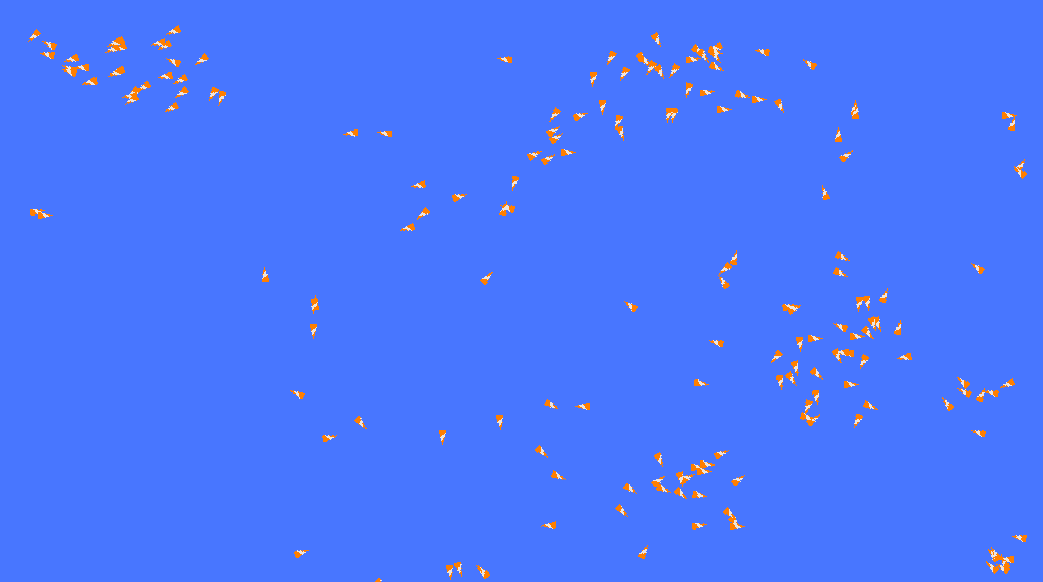
\includegraphics[width=0.6\textwidth]{flocking_example.png}
    \caption{Przykładowy wygląd kilku ławic w w których ryby zachowują do siebie dystans a także wyrównują swoją prędkość do sąsiadów.}
\end{figure}
\subsection{Porównanie z qlearningiem}
Podczas obserwowania symulacji zauważyliśmy, że kumulowanie wniosków z qtable razem z siłą sterującą w ławicy daje ciekawy efekt podczas uczenia. Mianowicie boidy odziałowują na siebie w każdej chwili, dlatego kiedy kilka boidów rozbijało się o krawędź, reszta ławicy która była za nimi zmieniała swój kierunek jednocześnie aktualizując znacznie większą część tablicy stanów.\\
Jednocześnie postanowiliśmy podać rybom zasadę, aby sugerowały się zarówno qlearningiem jak i ławicą kiedy nie widzą drapieżnika, natomiast samym qlearningiem jeśli drapieżnik jest w polu reakcji. Dało to interesujące wizualnie efekty, ponieważ kiedy jedna ryba unikała drapieżnika, reszta ławicy mimo że go nie widziała, dopasowywała swój ruch do uciekającej. 
\subsection{Pomiary}
W celu zmierzenia jak dokładnie radzą sobie ryby z podanym zachowaniem, uczyliśmy ryby oddzielnie z samym qlearningiem oraz z qlearningiem wspieranym przez zachowanie ławicowe. Ponieważ drapieżniki do tej pory również uczyły sie, a jednoczesne uczenie ryb i drapieżników nie pozwoliłoby zebrać znaczących pomiarów zmieniliśmy zachowanie zachowanie drapieżników. Drapieżnik kieruje się do najbliższej widocznej ryby, chyba że jest blisko granicy wtedy kieruje się ku środkowi planszy, a także drapieżniki wzajemnie odpychają się, aby zapobiec tłoczeniu się na środku planszy.

\begin{figure}[H]
    \begin{minipage}{0.48\textwidth}
        \centering
        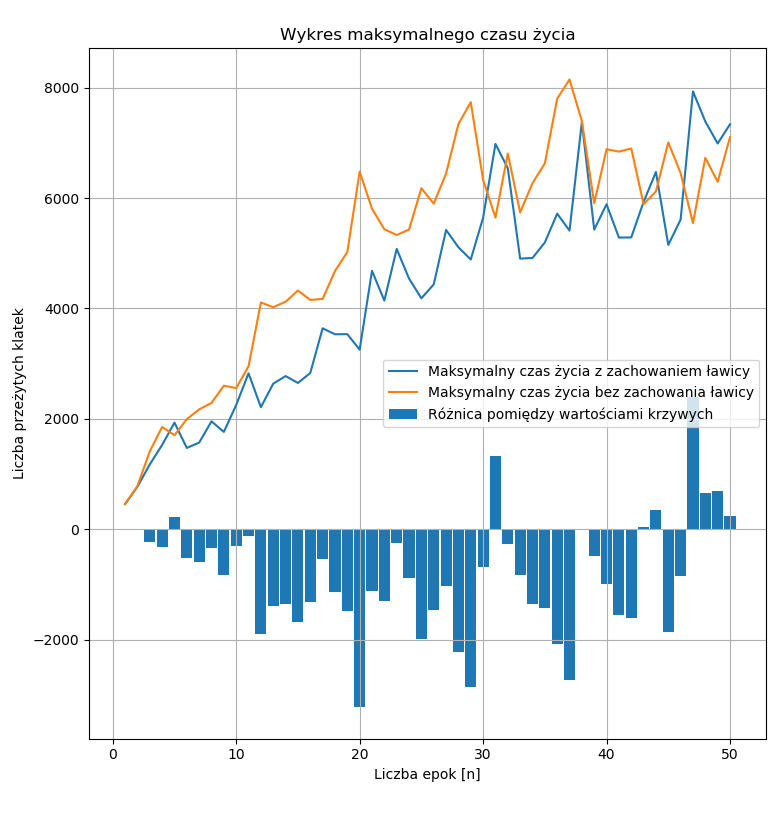
\includegraphics[width=\textwidth]{maximum_lifetime.png}
        \caption{Maksymalny czas życia przy kącie widzenia \(360^{\circ}\)} 
    \end{minipage}
    \hspace{0.02\textwidth}
    \begin{minipage}{0.48\textwidth}
        \centering
        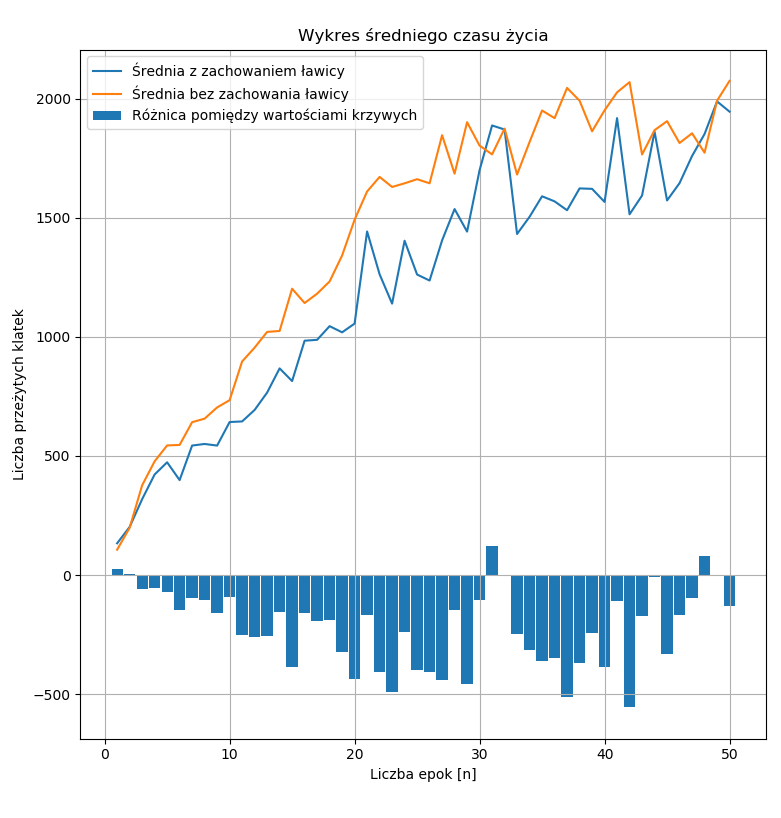
\includegraphics[width=\textwidth]{average_lifetime.png}
        \caption{Średni czas życia przy kącie widzenia \(360^{\circ}\)}
    \end{minipage}
\end{figure}
Pomiary zostaly dokonane poprzez uśrednienie wyników z 5 procesów uczenia. Jak widać wbrew oczekiwaniom ryby z zachowaniem ławicowym osiągają gorsze wyniki niż bez. Może to być efekt podanego pełnego kąta widzenia, ryby widzą za dużo i gubią się lub bez zachowania ławicy mogą lepiej wykorzystać pełną wizję. 
\begin{figure}[H]
    \begin{minipage}{0.48\textwidth}
        \centering
        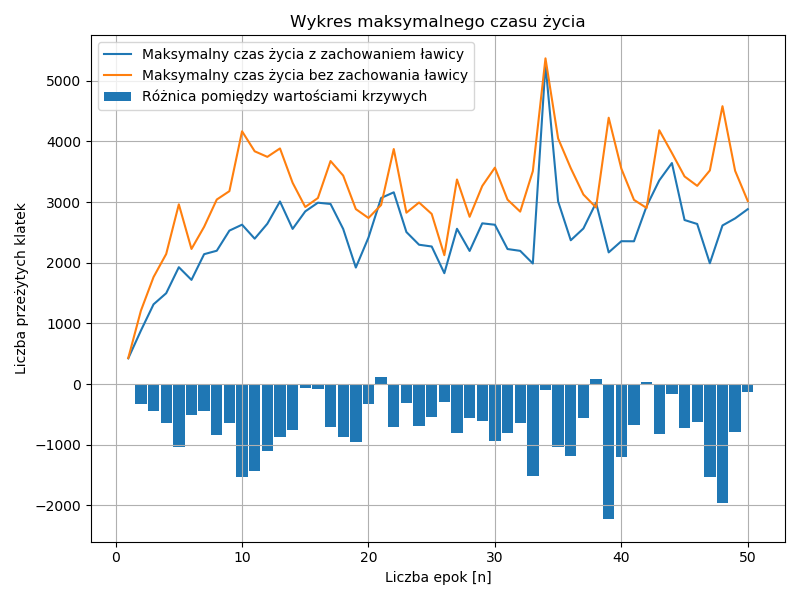
\includegraphics[width=\textwidth]{maximum_lifetime_angle_300.png}
        \caption{Maksymalny czas życia przy kącie widzenia \(300^{\circ}\)}
    \end{minipage}
    \hspace{0.02\textwidth}
    \begin{minipage}{0.48\textwidth}
        \centering
        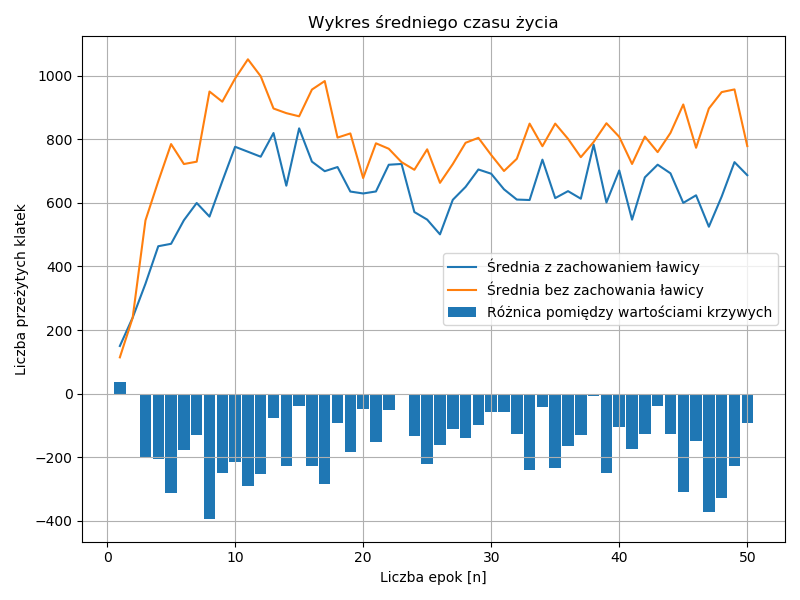
\includegraphics[width=\textwidth]{average_lifetime_angle_300.png}
        \caption{Średni czas życia przy kącie widzenia \(300^{\circ}\)}
    \end{minipage}
\end{figure}
Wbrew oczekiwaniom tutaj również przewagę ma czysty qlearning. Jest to interesujące ponieważ oczekiwanym wynikiem była przewaga zachowania ławicowego przez to że ryby nie widzą co jest za nimi, mogą jedynie reagować na zachowanie sąsiadów. Wprowadzenie algorytmu ławicowego daje bardzo ładne wrażenia wizualne, jednak wykres pokazuje że sztywne zachowanie w pewnych sytuacjach musi powodować ogłupienie boida, zatem stosując qlearning nie powinniśmy wprowadzać innych systemów decyzyjnych.
\section{Wnioski}
Qlearning jest ciekawą i prostą do zaimplementowania techniką uczenia, która nie wymaga w zasadzie żadnych zewnętrznych bibliotek, wystarczy jedna tablica i sposób jej aktualizowania. Bardzo dobrze radzi sobie z problemami w których można w jasny sposób określić akcję do wykonania, np poruszenie się o 2 metry w lewo lub 2 metry w prawo, wciśnięcie przycisku itp. Bardzo istotne jest też, aby charakterystyka rozwiązywanego problemu pozwalała na natychmiastowe określenie czy wykonana akcja była korzystna czy nie. Problem pojawia się kiedy zadanie osadzone jest w przestrzeni ciągłej, tak jak nasz problem boidów. O ile nie jest trudne zdyskretyzowanie wartości odpowiadających za stan (chociaż wprowadza to kolejne hiperparametry), bardzo problematyczne staje się wyznaczenie akcji, ponieważ nie jest możliwe otrzymanie konkretnej wartości. Zamiast tego konieczne jest wprowadzanie zmian w iterpretacji wybranej akcji, tak jak zrobiliśmy to w sekcji \ref{sec:politics_modification}. Co więcej w przestrzeni ciągłej trudne jest określenie natychmiastowego skutku akcji i wymaga to modyfikowania głównego równania (\ref{eqn:bellman_equation}) używanego do aktualizacji tablicy stanów.

Technika jednak dała podłoże pod dalszy rozwój uczenia ze wzmocnieniem. W tradycyjnym sposobie używamy tabeli Q, która jest funkcją stanu i akcji i przewiduje nagrody. Zamiast tabeli możliwe jest użycie głębokich sieci neuronowych, które przy odpowiedniej architekturze mogą dokladniej nauczyć się przewidywać wartości nagród. Ponieważ qlearning słabo radzi sobie z przestrzenią ciągłą, dobrym rozwiązaniem może być też technika Deep Deterministic Policy Gradient, która polega na zapamiętywaniu kolejnych stanów, a ocena następuje po zakończeniu epoki. Wtedy polityka która przyniosła większe zyski jest maksymalizowana, a polityka słaba minimalizowana. Powoduje to zbieganie się do optymalnego sposobu działania i rozwiązuje problem opóźnionej gratyfikacji.
\end{document}